\documentclass[12pt, a4paper, twoside]{report}
\usepackage[utf8]{inputenc}
\usepackage[T1,T2A]{fontenc}

\usepackage[russian, english]{babel}
\usepackage{xcolor} %for transparency
\usepackage{graphicx}

\usepackage{indentfirst}

\newcommand{\HRule}{\rule{\linewidth}{0.5mm}}
%\setcounter{section}{1}
\renewcommand{\thesection}{\arabic{section}}

%Rename contents - magic here
\addto\captionsenglish{% Replace "english" with the language you use
	  \renewcommand{\contentsname}%
	      {Оглавление}%
      }
%END rename contents
      \usepackage[top=2.5cm, left=2.5cm, right=2.5cm]{geometry}
      \usepackage{amsmath, amsfonts, amsthm, amssymb}

\begin{document}

\begin{titlepage}
\begin{center}
\fontencoding{T1}\selectfont

\textsc{\LARGE Liceum Boarding School number 2}\\[1.5cm]

\textsc{\Large Some crappy project}\\[0.5cm]

% Title
\HRule \\[0.4cm]
{ \huge \bfseries Tesseract and hyperplane investigation\\[0.4cm] }

\HRule \\[1.5cm]

% Author and supervisor
\noindent
\begin{minipage}{0.4\textwidth}
\begin{flushleft} \large
\emph{Authors:}\\
Ilgic \textsc{Mustafin} \newline
\fontencoding{T2A}\selectfont
Гриша \textsc{Maxxx} \newline %USE RUSSIAN FONT
\fontencoding{T1}\selectfont %USE LATIN HERE
Mirolin \textsc{M} 
and \newline
Arthur \textsc{Nugmanov} 
\end{flushleft}
\end{minipage}%
\begin{minipage}{0.4\textwidth}
\begin{flushright} \large
\emph{Supervisor:} \\
Marsel \textsc{Abiy}
\end{flushright}
\end{minipage}

\vfill

% Bottom of the page
{\large \today}

\end{center}
\end{titlepage}
 %Load titlepage so we do not mess up the numeration

\tableofcontents

\newpage
\section{Введение}
Введение, тезисы, примерное описание работы.
Наше исследование ставит своей целью разработать программу, которая с помощью введенных данных строит сечение четырехмерного куба - тессеракта трехмерной гиперплоскостью. А также описание работы программы, и ее математическое обоснование. Нами была разработана программа на языке Java, использующая 4 введенные точки в четырехмерном пространстве или вектор и точку для построения трехмерного тела – сечения тессеракта. 
Для четырехмерного пространства была использована аналогия метода нахождения точек сечения куба плоскостью и метода поворота плоскости в трехмерном пространстве.

Как известно, гиперкуб представляет собой куб в четырехмерном пространстве, может также называться тетракубом и тессерактом. В данной работе будет рассматриваться представление данной фигуры в виде множества точек в Евклидовом пространстве $(\pm 1,\pm 1,\pm 1, \pm 1)$. Тессеракт ограничивают 8 гиперплоскостей, т.е. подпространств, на единицу меньшей, чем объемлющее пространство.

\begin{figure}[h!]
	\center
	\framebox{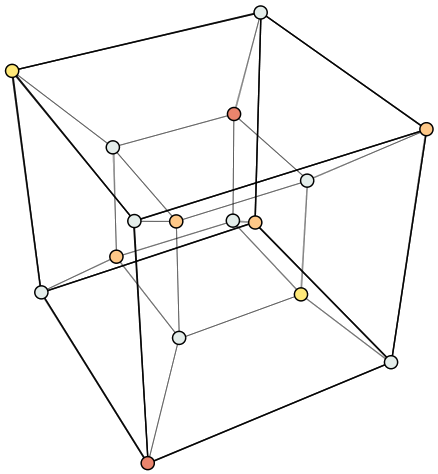
\includegraphics[scale=0.5]{./tesseract_fig1.png}}
	\clearpage
\end{figure}
\section{Тессеракт, или четырехмерный гиперкуб}
Конечно, невозможно представить графически, как будет выглядеть данный гиперкуб в четырехмерном пространстве, не выходя из трехмерного. Можно лишь представить проекцию данного тессеракта на трехмерную плоскость. В случае проекции невозможно определить точки сечения, поэтому все действия нами выполнялись в четырехмерных координатах для получения трехмерного сечения, представляющего из себя многогранник.

Далее будет рассмотрен довольно простой способ представления проекции тессеракта на трехмерную плоскость. Этот алгоритм позволяет представить примерно, как выглядит рабочий куб, но, как уже отмечалось выше, он не позволяет определить точки пересечения гиперплоскости с четырехмерным кубом.
\subsection{Построение проекции гиперкуба на плоскость}
Попытаемся представить себе, как будет выглядеть гиперкуб, не выходя из трёхмерного пространства. Возьмем одномерное пространство (линию), выделим на нем отрезок длиной $а$. Теперь перенесем его на двумерную плоскость и на расстоянии $а$ от него нарисуем параллельный ему отрезок той же длины, затем соединим концы. Получится квадрат. Повторив эту операцию с двумерной плоскостью, получим трехмерный куб, а если применить ту же операцию к трехмерному пространству, то получится гиперкуб т.е. его можно представить, как два трехмерных куба, лежащих в параллельных трехмерных пространствах, с попарно соединенными вершинами.

\begin{figure}[h!]
	\framebox{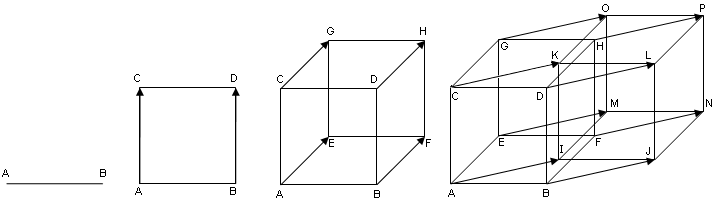
\includegraphics[scale=0.6]{./make_tess.png}}
	\clearpage
\end{figure}

Как видим, отрезок $AB$ в результате параллельного переноса превращается в квадрат, т.е. уже куб 2 измерения. По аналогии куб $ABCDEFGH$ образует проекцию гиперкуба на трехмерную плоскость.

Если задуматься о том, как будет выглядеть сечение тессеракта в четырехмерном пространстве, можно прийти к следующей аналогии: сечением одномерного объекта будет точка, двумерного -  отрезок, трехмерного - плоскость. По аналогии сечением четырехмерного объекта является трехмерный объект. Наша задача состоит как раз в отыскании принципа построения данных сечений.

\section{Описание работы программы, скриншоты и прочие особенности}
\subsection{Возможности программы}
Данная программа предназначена для визуализации отображения четырехмерного объекта тессеракта на трехмерную плоскость и определения сечения по заданным данным. Для достижения этой цели использовался алгоритм, описанный ниже в пункте "Алгоритм работы программы, его математическое описание". \\
Как уже было сказано, использовался язык JAVA 7 по причине того, что данный язык программирования представляет возможности очень быстрого прототипирования и разработки программного продукта, в то же время оставаясь как в высокой степени понятным и дочтаточно легко понимаемым человеком, так и кроссплатформенным. \\
После написания основного алгоритма и логики работы стала задача составить графический интерфейс, для которого была использована графическая библиотека JAVA Swing. Таким образом, перейдем к рассмотрению основных возможностей программы на примере графического интерфейса пользователя:
\\

\framebox{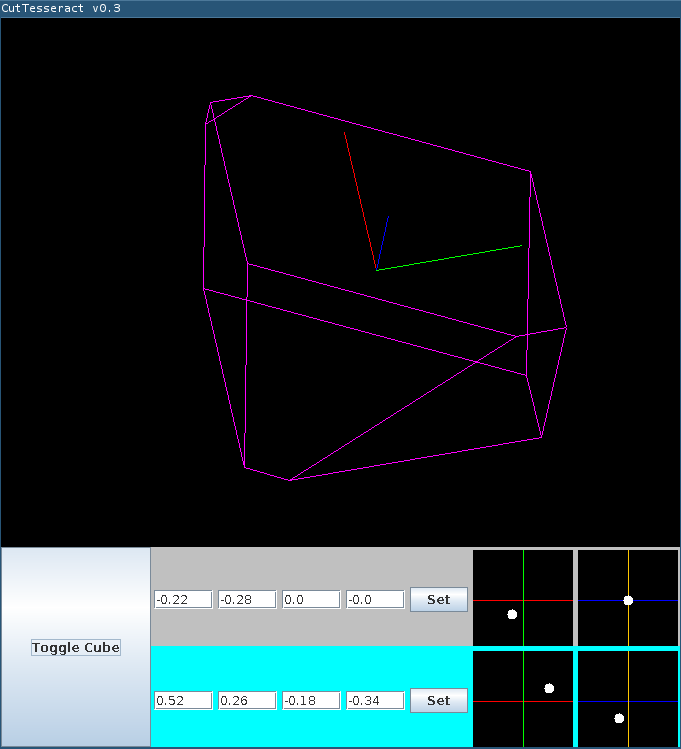
\includegraphics[scale=0.6]{./post3.png}}

Главное пространство занимает геометрическая трехмерная модель тессеракта(белые линии) и вписанного в него сечения (на данном скриншоте тессеракт не показан). Ниже панели отображения расположена панель управления, задающая произвольное сечение точкой и вектором нормали. Серая панель задает координаты и местоположение точки относительно основных координатных осей, тогда как голубая панель задает вектор. Как понятно из скриншота, задать точку и вектор, используя графическое окружение можно двумя способами: непосредственно ввести координаты в поля ввода и нажать кнопку Set, или же использовать для введения специальные квадратные области графического задания координат. 

\section{Алгоритм работы программы, его математическое обоснование}
Перейдем к описанию алгоритма построения сечений.

Для начала нужно задать уравнение гиперплоскости сечения. Для этого нужно либо 4 четырехмерные точки, либо четырехмерный вектор и точку. Таким образом, задается гиперплоскость сечения. После получения уравнения гиперплоскости сечения алгоритм проводит проверку каждого ребра куба на пересечение с гиперплоскостью сечения. Далее проверяем, если точки сечения лежат на одной грани, то можно их соединить (создать из них сегмент), после чего отображаем полученные сегменты на экране по двум точкам и получаем финальное сечение. Однако, оно все еще в четырехмерных координатах, поэтому нормаль гиперплоскости сечения вместе с сечением нужно повернуть так, чтобы она стала параллельна четвертой оси координат (0, 0, 0, 1). Для достижения данной задачи нами используются матрицы поворота, о которых будет сказано в дальнейшем. В результате этих манипуляций четвертая координата у всех точек сечения становится одинаковой, т.е. её можно не учитывать при выводе полученных граней сечения на экран. После этого сечение представляет собой трехмерное геометрическое тело, вполне доступное для наблюдения и понимания.

Разберем подробнее процесс задания уравнения гиперплоскости сечения.
\subsection{Уравнение гиперплоскости сечения}
Как было сказано, мы используем два метода для решения данной задачи. Разберем, как задается уравнение гиперплоскости по четырем 4D точкам.
Известно, что уравнение искомой плоскости записывается в виде:
$$ax + by + cz + dw + e=0,$$ где $(a,b,c,d,e)$ - коэффициенты, а $(x,y,z,w)$ - координаты возможных точек. Точка принадлежит гиперплоскости, если выполняется равенство.

Требуется по данным точкам $$A(x_1,y_1,z_1,w_1), B(x_2,y_2,z_2,w_2), C(x_3,y_3,z_3,w_3), D(x_4,y_4,z_4,w_4)$$ составить уравнение гиперплоскости, т.е. найти нужные коэффициенты.

Уравнением плоскости будет являться решением данной матрицы: $$ \left|
		\begin{array}{cccc}
			x-x_1 & y-y_1 & z-z_1 & w-w_1     \\
			x_2-x_1 & y_2-y_1 & z_2-z_1 & w_2-w_1    \\
			x_3-x_1 & y_3-y_1 & z_3-z_1 & w_3-w_1      \\
			x_4-x_1 & y_4-y_1 & z_4-z_1 & w_4-w_1 
		\end{array}
	\right|=0

$$

Далее разберем другой способ. Пусть нам даны точка $A(x_1,y_1,z_1,w_1)$, и вектор $\vec N(x_2,y_2,z_2,w_2)$. С помощью них мы можем задать уравнение гиперплоскости $P(ax + by + cz + dw + e=0)$.
Вектор $N$ будет являться нормалью к данной плоскости, т.е. будет справедливо следующее равенство: $$a=x_2, b=y_2, c=z_2, d=w_2.$$ Останется найти коэффициент $e$, который будет находиться подстановкой координат данной точки $A$ в уравнение гиперплоскости. Т.е. $$e=-(x_2x_1+y_2y_1+z_2z_1+w_2w_1)$$
Таким образом, мы нашли гиперплоскость, используя введенные данные.
\subsection{Нахождение пересечения гиперплоскости сечения с ребрами гиперкуба}
Для нахождения точек сечения надо найти пересечения данной гиперплоскости $P$ и всех ребер куба.
Допустим, имеем гиперкуб с координатами $$(\pm1, \pm1, \pm1, \pm1),$$ 16 вершин или 32 ребра. Для начала проверим, являются ли вершины гиперкуба точками сечения. Для этого берем последовательно все 16 вершин гиперкуба и подставляем их координаты в уравнение гиперплоскости.
\newline
$\begin{equation}
A(x_1,y_1,z_1,w_1) \\
P(ax + by + cz + dw + e = 0) \\
\left[
	\begin{array}{ccc}
		ax_1 + by_1 + cz_1 + dw_1 + e = 0 & \mbox{Вершина гиперкуба принадлежит сечению} 
		\\
		ax_1 + by_1 + cz_1 + dw_1 + e > 0 & \mbox{Вершина гиперкуба лежит выше плоскости сечения}
		\\
		ax_1 + by_1 + cz_1 + dw_1 + e < 0 & \mbox{Вершина гиперкуба лежит ниже плоскости сечения} 
	\end{array}
\end{equation}$
\\

Теперь, если данные точки, принадлежащие одному ребру, лежат по разные стороны от сечения, то между ними есть точка, принадлежащая сечению. Если обе точки лежат по одну сторону от сечения, то значит, данное ребро и плоскость сечения не имеют общих точек. Возможна также ситуация, когда вершина гиперкуба сама является точкой сечения.
\newpage
Обратимся к случаю, когда данные точки лежат по разные стороны от сечения. Требуется найти точку пересечения секущей гиперплоскости и данного ребра. Пусть мы работаем с ребром $AB$ гиперкуба и плоскостью сечения $P(ax + by + cz + dw + e = 0)$, для которой мы точно знаем, что она имеет общую точку с ребром.
\\
$\begin{equation}
A=(x_1,y_1,z_1,w_1)\\ 
B=(x_2,y_2,z_2,w_2) \\
\vec{AB}=((x_2-x_1),(y_2-y_1),(z_2-z_1),(w_2-w_1))
\end{equation}$

\\
Зададим параметрическое уравнение прямой $AB$ через точку $A$ и вектор $\vec{AB}$.
\\
$
\begin{equation}
	A(x_1,y_1,z_1,w_1) \\
	\vec{AB}=(a_x,a_y,a_z,a_w) \\
	\left\{
		\begin{array}{ccc}
			x=x_1+a_xt \\
			y=y_1+a_yt \\
			z=z_1+a_zt \\
			w=w_1+a_wt
		\end{array}
\end{equation}
$

\\
Требуется найти неизвестный коэффициент $t$. Находим его следующим образом, используя уравнение гиперплоскости:
\\
$$	P(ax+by+cz+dw+e=0)$$ 
$$	t=-\frac{(ax_1+by_1+cz_1+dw_1+e)}{(aa_x+ba_yca_z+da_w)}$$

Теперь параметрическое уравнение задано, требуется найти координаты точки пересечения данного ребра с полученной прямой. Для нахождения координат точек пересечения нужно вычислить значения $(x,y,z,w)$, входящие в состав системы параметрического уравнения прямой. Найденная точка лежит между вершинами данного ребра тессеракта и принадлежит гиперплоскости сечения. 

Требуется повторить данную операцию для всех 32 ребер, которые имеют общие точки с данной плоскостью сечения.
\subsection{Построение геометрического тела сечения, поворот}
После нахождения всех точек, требуется соединить их ребрами. Для этого перебираем все возможные пары точек из полученного множества. Для каждой пары применим следующие критерии нахождения их на одном ребре - чтобы две данные точки лежали на одном ребре, необходимо, чтобы хотя бы две их координаты были одинаковы и равны соответственно $1$ и $-1$.
Если такое условие выполняется, то две данные полученные точки можно соединить ребром. Множество полученных ребер и будет ограничивать все множество точек полученного сечения.

Следующим шагом требуется повернуть плоскость сечения таким образом, чтобы нормаль к данной плоскости стала параллельной четвертой координатной оси $Ow$. Для осуществления данной цели используются матрицы поворота точки в плоскостях. Составляя нужную композицию поворотов, можно достичь поставленной выше задачи.

Пусть дана система координат $Oxyzw$. Определим матрицы поворота относительно плоскостей:
\\

$
M_{xy}(\alpha)=
\begin{equation}
	\left(
		\begin{array}{cccc}
		\cos \alpha & -\sin \alpha & 0 & 0 \\
		\sin \alpha & \cos \alpha & 0 & 0 \\
		0 & 0 & 1 & 0 \\
		0 & 0 & 0 & 1
	\end{array}\right)
\end{equation}
$
\\ 

$
M_{xz}(\alpha)=
\begin{equation}
	\left(
		\begin{array}{cccc}
		\cos \alpha & 0 & \sin \alpha & 0 \\
		0 & 1 & 0 & 0 \\
		-\sin \alpha & 0 & \cos \alpha & 0 \\
		0 & 0 & 0 & 1
	\end{array}\right)
\end{equation}
$
\\

$
M_{yz}(\alpha)=
\begin{equation}
	\left(
		\begin{array}{cccc}
		1 & 0 & 0 & 0 \\
		0 & \cos \alpha & -\sin \alpha & 0 \\
		0 & \sin \alpha & \cos \alpha & 0 \\
		0 & 0 & 0 & 1
	\end{array}\right)
\end{equation}
$
\\

Определим произвольную матрицу поворота $M(\phi)$ как композицию поворотов $$M(\phi)=M_{xy}(\alpha)\circ M_{xz}(\beta)\circ M_{yz}(\gamma)$$.
Таким образом, чтобы повернуть нормаль плоскости сечения параллельно $Ow$, нам потребуется повернуть последовательно в плоскостях $xy, xz, yz$.

После данных манипуляций получаем трехмерное результирующее сечение, которое и выводится на экран. Данное сечение не имеет координаты $w$, и, как следствие, представляет собой геометрическое тело в трехмерном Евклидовом пространстве.
Данное сечение имеет одинаковую координату $w$, и, как следствие, идентично со своей проекцией на трехмерное пространство.

\section{Заключение}
Таким образом, наше исследование ставило своей целью создание программы, которая может изобразить трехмерное сечение гиперкуба, поворачивать его, используя формулы поворота точки относительно начала координат, математическое обоснование правильной работы программы и описание её работы. Данная задача была нами достигнута.
\section{Список используемой литературы}
https://ru.wikipedia.org/wiki/%D0%A2%D0%B5%D1%81%D1%81%D0%B5%D1%80%D0%B0%D0%BA%D1%82 \\
----- \\
http://www.coolreferat.com/%D0%9A%D0%BE%D0%BC%D0%BF%D1%8C%D1%8E%D1%82%D0%B5%D1%80%D0%BD%D0%BE%D0%B5_%D0%BF%D1%80%D0%B8%D0%BB%D0%BE%D0%B6%D0%B5%D0%BD%D0%B8%D0%B5_%D0%A1%D0%B5%D1%87%D0%B5%D0%BD%D0%B8%D0%B5_%D0%BC%D0%BD%D0%BE%D0%B3%D0%BE%D0%B3%D1%80%D0%B0%D0%BD%D0%BD%D0%B8%D0%BA%D0%BE%D0%B2_%D1%87%D0%B0%D1%81%D1%82%D1%8C=3
\section{Приложения}
Программный код. Компилировать на Java 7 \\
Программу можно скачать с созданного репозитория по адресу: \\
http://imustafin.github.io/CutTesseract/ \\
\end{document}

